\newpage
\section{РЕАЛИЗАЦИЯ} 

\subsection{Технологии и библиотеки} 

Для решения поставленной задачи использовались следующие технологии:

\begin{itemize} 
  \item HTML5 -- язык разметки, используемый для построения структуры и представления веб-страниц. 
    Это пятая версия языка, которая добавляет поддержку тэга \textless{}canvas\textgreater{}, 
    который позволяет попиксельному отображение изображений через различные контексты. 
    На момент написания работы, доступно два основных контекста: 2D и WebGL.

    2D был первым реализованным типом контекста. Он реализован как конечный автомат (схоже 
    с OpenGL) и может быть использован для высокопроизводительной визуализации двухмерных объектов, 
    таких как линии, прямоугольники, кривые, bitmap-изображения и т.д.

    Следующий тип контекста позволил разработчикам создавать высокопроизводительные 3D изображения 
    без использования сторонних плагинов и расширений. Это значит что пользователям не требуется 
    устанавливать дополнительное ПО (например, Adobe Flash Player или Java VM) для просмотра. 
    Кроме того, WebGL контекст позволяет работать с программируемым графическим конвейером. 

  \item JavaScript -- динамический язык программирования. Используется для взаимодействия с 
    пользователями, управлением веб-страницей и асинхронной загрузки ресурсов.

  \item Coffeescript -- язык программирования, который транслируется в JavaScript. Добавляет 
    синтаксический сахар для повышения краткости и читаемости кода. Например, классы 
    (из объектно-ориентированного программирования), которые имеют четкую и понятную структуру.

  \item WebGL -- спецификация интерфейса для создания динамичных 2D и 3D сцен без использования 
    сторонних плагинов. Создан и поддерживается организацией Khronos Group, на данный момент, 
    разрабатывающей спецификацию OpenGL. WebGL служит связкой между высокоуровневым языком 
    JavaScript и низкоуровневыми операциями на графических процессорах.

  \item GLSL (OpenGL Shading Language) -- язык высокого уровня для программирования шейдеров. 
    Основным преимуществом GLSL является переносимость между платформами и ОС. Т.е. алгоритмы, 
    описанные в рамках данной работы, могут быть перенесены на другие платформы без изменения 
    кода программы.
\end{itemize}

Для упрощения разработки используется библиотека Zepto.js. Она упрощают работу с AJAX запросами, 
которые используются для загрузки ресурсов. Является минималистичным аналогом jQuery, 
который также может являться альтернативой.

Основным преимуществом данного подхода к реализации является кроссплатформенность и быстрота 
разработки.

\subsection{Общая архитектура}

Первая задача, которую необходимо решить при реализации -- организация структуры таким образом, 
чтобы добавление и расширение существующих компонентов было максимально простым. Задача
усложняется, когда появляется большая зависимость между компонентами. Схема зависимостей
между компонентами системы изображена на рисунке \ref{fig:architecture}.

\begin{figure}
\begin{center}
  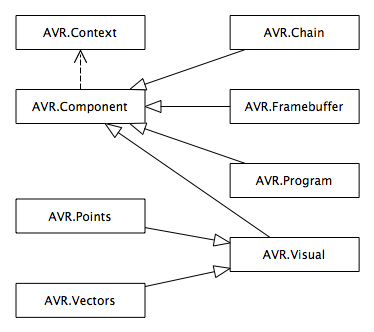
\includegraphics[scale=1]{Figures/architecture}
\end{center}
\caption{Схема зависимостей между компонентами}
\label{fig:architecture}
\end{figure}


В состав программного обеспечения входят следующие компоненты:

\begin{itemize}
  %\item автоматическая инициализация контекста WebGL с выставлением
    %необходимых аттрибутов для вычислений и визуализации;
  \item компонент для загрузки и компиляции шейдерных программ с расширением
    функциональности;
  \item инструмент для составления проходов и передачи данных между кадровыми буферами и 
    программами;
  \item компонент визуализации;
\end{itemize}

Основой всей программы служат два класса: 

\begin{itemize}
  \item AVR.Context -- является компонентом инициализации, загрузки и создания ресурсов.
  \item AVR.Component -- задачи которого сводится к связь компонентов с контекстом.
\end{itemize}

AVR, в данном случае, это объект находящийся в глобальном объекте window. Используется 
как пространство имен для всех классов программы. 

Каждый компонент системы реализован в виде отдельного класса, наследующего свойства 
AVR.Component. Для удобства инициализации используется расширение объекта AVR.Context
через свойство prototype.

% webgl - автомат с состояниями, задача использования и освободжения ресурсов (кадровые буферы, 
% программы) -> сократить количество строчек => упрощение написания подобных программ.
% концепция языка js с обратными вызовами => использовать как контексты (в контексте данного
% колбэка активна такая-то программа, такой-то фреймбуфер. вне колбэка все освобождается

Следующая задача, которую необходимо решить -- работа с WebGL. WebGL реализован как конечный
автомат. Таким образом требуется постоянный контроль за тем, какие ресурсы сейчас активны. Это
значительно усложняет написание и увеличивает количество строк кода. Для решения данной задачи
за основу взята событийно-ориентированная парадигма языка JavaScript. 
Например, в метод для активации шейдерной программы передается функция, которая
вызывается после активации программы. Перед сменой программы запоминается уже активная. 
После успешного выполнения функции, сохраненная программа снова становится активной (рисунок \ref{fig:callback}).
Таким же образом реализована работа с текстурами и кадровыми буферами.

\begin{figure}
\begin{center}
  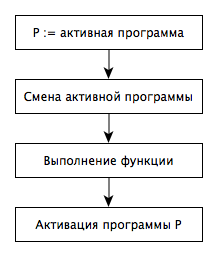
\includegraphics[scale=1]{Figures/callback}
\end{center}
\caption{Использование обратного вызова для активации шейдерных программ}
\label{fig:callback}
\end{figure}


Составление проходов и передача данными между кадровыми буферами реализована с помощью
компонента AVR.Chain, где описывается какая программа должна быть активна, в какой
кадровый буфер будет записан результат и значения каких кадровых буферов подаются на вход
фрагментного шейдера.

Для удобства работы с двойными кадровыми буферами (когда требуется чтобы хранилось предыдущее
состояние и новое) реализована система селекторов. Механизм работы следующий: при инициализации
указывается тип буфера (одиночный или двойной). Когда необходимо указать в какой буфер сохранятся 
или из какого будут извлекаться данные, указывается название буфера и один из селекторов:

\begin{itemize}
  \item Взять первый буфер (ключевое слово left)
  \item Взять второй буфер (ключевое слово right)
  \item Автоматически сменить и взять новый буфер (ключевое слово switch)
  \item Взять последний буфер (ключевое слово auto)
\end{itemize}

Расширение функциональности шейдеров заключается в виде предварительной обработки
и поиска директив. Реализована передача констант из основной программы и включение
кода других шейдеров в текущий. После предварительной обработки, код попадает на компиляцию
в WebGL. При необходимости в консоль браузера выводятся ошибки компиляции.

Компонент визуализации реализован в виде класса AVR.Visual. Каждый тип визуального представления
является классом, наследующим свойства AVR.Visual.

\subsection{Визуальные представления}

%\subsubsection{Точки и вектора в трехмерном пространстве}

Первая проблема с которой приходится сталкиваться -- как вывести данные хранящиеся в кадровом
буфере на экран. Для этого можно сначала вывести данные на ЦП, затем загрузить в вершинный буфер.
Недостатки данного решения:

\begin{itemize}
  \item Передача данных между центральным процессором и графическим занимает значительное
    количество времени. Ровно как и создание вершинного буфера.
  \item Ограничение стандарта WebGL при считывании данных с кадрового буфера: разрешается
    вывод только четырехмерного байтового вектор. Что означает потери при дискретезации.
\end{itemize}

Другой вариант -- перед началом визуализации создать вершинный буфер, содержащий UV-координаты
частиц в кадровом буфере. Таким образом исключается необходимость передавать данные
между процессорами и заново создавать вершинные буферы. При этом размеры буферов будут
сопоставимы с размерами кадровых буферов.

В спецификации WebGL есть несколько режимов отображения вершин: точки, линии, треугольники и т.д.
В данном типе визуализации используются отображения точек и линий (gl.POINTS и gl.LINES соответственно).

Исходные данные, необходимые для создания визуализации:

\begin{itemize}
  \item положения частиц;
  \item цветовая характеристика: по положению, по указателю, по другим параметрам симуляции 
    (например распределение плотности или вектора градиентов давления);
  \item направление векторов (для отображения векторного визуального представления);
\end{itemize}

Реализация визуализации векторов аналогична точкам с некоторыми изменениями: для отображения
одной частицы требуется не одна, а две вершины. Это значит что размер вершинного буфера
будет в два раза больше и хранить не только UV-координаты, но и флаг обозначающий начало
и конец вектора. В качестве флага можно использовать z-координату.

Алгоритм вершинного шейдера:

\begin{enumerate}
  \item По UV-координате частицы считывается информация о текущем положении частицы.
  \item По третьей координате определяется начало и конец вектора.
  \item При необходимости считывается информация о направлении вектора и добавляется к
    текущему положению частицы.
  \item Полученная вершина проходит через матрицу трансформации для создания перспективы.
\end{enumerate}

Во фрагментном шейдере в зависимости от необходимой цветовой характеристики считываются
соответствующие данные из вершинного шейдера и кадровых буферов и передаются на выход.
Для векторов на вход программы подается начальный и конечный цвет, которые
интерполируются в зависимости от текущего фрагмента.

Результат визуализации в виде точек и векторов изображены на рисунках \ref{fig:ss_points} и
\ref{fig:ss_vectors} соответственно.


\begin{figure}
\begin{center}
  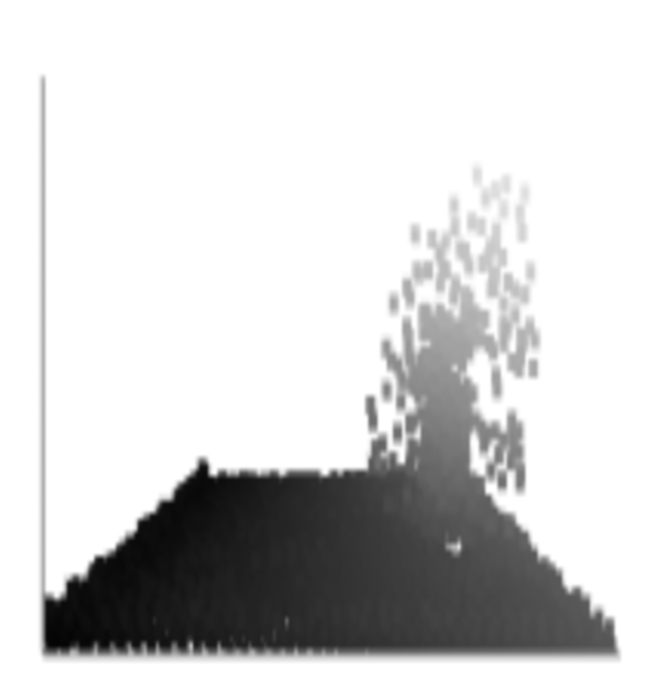
\includegraphics[scale=1]{Figures/points}
\end{center}
\caption{Визуализация в виде точек}
\label{fig:ss_points}
\end{figure}

\begin{figure}
\begin{center}
  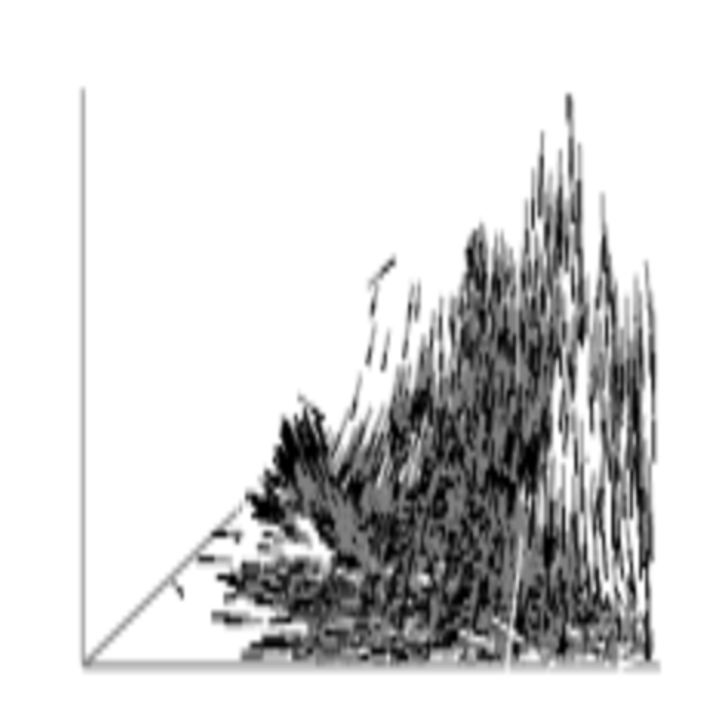
\includegraphics[scale=1]{Figures/vectors}
\end{center}
\caption{Визуализация в виде векторов}
\label{fig:ss_vectors}
\end{figure}


%\subsubsection{Шагающие кубики}
% ???? 

\subsection{Взаимодействие пользователя с симуляцией}

Одним из критериев к инструменту является интерактивность.
Необходимо максимально облегчить разработку части, где программист описывает логику 
реакции на входящие изменения.

В частности, работа с константами в шейдерных программах реализована
таким образом, что при обновлении одной величины, автоматически перестраивается
вся визуализация.

\subsubsection{Смена углов обзора}

По-умолчанию при использовании одного из встроенных типов представлений,
строится сцена с координатной сеткой. Пользователь, нажимая на клавиши
или кнопки на экране может вращать, изменять масштаб визуализации.

В данной работе это реализовано с помощью матрицы преобразования,
которая умножается на конечный вектор. Матрица формируется в JavaScript 
коде, затем передается в скомпилированные шейдерные программы.

Матрица задается следующим образом:

\begin{equation}
\label{eq:}
  M = R_x * R_y * S,
\end{equation}

где \\

\begin{equation}
\label{eq:}
  S = 
  \begin{bmatrix}
    S_x & 0 & 0 & 0 \\
    0  & S_y & 0 & 0 \\
    0  & 0 & S_z & 0 \\
    0 & 0 & 0 & 1
  \end{bmatrix}
\end{equation}

\begin{equation}
\label{eq:}
R_x = 
\begin{bmatrix}
  1 & 0 & 0 & 0 \\
  0 & cos(\theta) & -sin(\theta) & 0 \\
  0 & sin(\theta) & cos(\theta) & 0 \\
  0 & 0 & 0 & 1
\end{bmatrix}
\end{equation}

\begin{equation}
\label{eq:}
R_y = 
\begin{bmatrix}
  cos(\theta) & 0 & sin(\theta) & 0 \\
  0 & 1 & 0 & 0 \\
  -sin(\theta) & 0 & cos(\theta) & 0 \\
  0 & 0 & 0 & 1
\end{bmatrix}
\end{equation}

Далее перспектива строится присвоением координаты $z$ четвертой компоненте
вектора. Это создает эффект "удаления".

\subsubsection{Воздействие на частицы методом отбрасывания лучей}

Подобно предыдущему способу взаимодействия, строится обратный процесс. 
Преобразование происходит из двумерных координат в трехмерные.

Необходимо умножить матрицу преобразования на координату каждой из частиц. 
Затем вдоль координаты $z$ направленной от наблюдателя в заданном радиусе
выбираются частицы на которые будет воздействовать какая-то сила (\ref{fig:user_input}). 
Это делается при помощи подставления уже двумерных координат частицы в 
уравнение окружности.


\begin{figure}
\begin{center}
  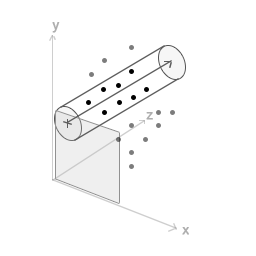
\includegraphics[scale=1.0]{Figures/user_input}
\end{center}
\caption{Определение задействованных точек}
\label{fig:user_input}
\end{figure}

\subsection{Реализация демонстрационного примера}

Выбор данного примера для демонстрации обоснован относительной сложностью реализации
и требовательностью к производительности при большом количестве частиц.

\subsubsection{Гидродинамика сглаженных частиц}

Гидродинамика сглаженных частиц (англ. Smoothed Particle Hydrodynamics, SPH) -- вычислительный 
метод, используемый для симуляции флюидов.

Флюид -- текучие вещества. К ним можно отнести:
\begin{itemize}
  \item жидкости. Примером жидкости может служить вода, масло, и т.д.;
  \item газы. Плотность данной среды меньше чем жидкостей. Пример: воздух;
  \item плазма;
\end{itemize}

Симуляция флюидов обычно описывается уравнениями Навье-Стокса \cite{sphHarada}.
Они являются одними из важнейших в гидродинамике и применяются в математическом
моделировании природных явлений и технических задач.

\begin{equation}
\label{eq:nve1}
  \rho[\frac{\delta{}v}{\delta{}t} + v \bullet \bigtriangledown{}v] = \rho{}g - \bigtriangledown{}p + \mu{}\bigtriangledown^2v
\end{equation}

\begin{equation}
\label{eq:massCont}
  \rho(\bigtriangledown\bullet{}v) = 0
\end{equation}

Двигаясь за счет гравитации $g$, давления $\bigtriangledown{}p$ и скорости $\mu\bigtriangledown^2v$ частицы жидкости движутся из зоны высокого давления в зону низкого.

Еще один параметр который влияет на поведение флюидов -- вязкость $\mu$.
Примером текучего вещества с низкой вязкостью может являться вода, воздух.
С высокой: мед, грязь. \\

В данной работе рассмотрен упрощенный случай: симуляция несжимаемого потока
Ньютоновских флюидов. Уравнение \eqref{eq:nve1} описывает состояние жидкости.

Составляющие уравнения:

\begin{itemize}
  \item $\rho$ -- плотность (скалярная величина);
  \item $p$ -- давление (скалярная величина);
  \item $g$ -- вектор гравитации;
  \item $v$ -- вектор скорости;
\end{itemize}

Давление $p$ может быть представлено как

\begin{equation}
\label{eq:pressure}
  p = k(\rho - \rho_0),
\end{equation}

где $\rho_0$ -- плотность вне флюида. \\

Уравнение \eqref{eq:massCont} может быть выполнено при условии что масса частиц
постоянна и частицы ниоткуда не создаются и никуда не исчезают.

Конечный вид уравнения для каждой частицы принимает вид:

\begin{equation}
\label{eq:}
\frac{dv_i}{dt} = g - \frac{1}{\rho_i}\bigtriangledown{}p + \frac{\mu}{\rho_i}\bigtriangledown^2v
\end{equation}

Суть вычислительного метода гидродинамики сглаженных частиц состоит в аппроксимации величин
уравнений Навье-Стокса с использованием функции сглаживающего ядра.

\begin{equation}
\label{eq:mon1992}
A_i(r) = \int{}A(r')W(r - r', h)dr' \approx \sum_{b}A(r_b)W(r - r_b, h)
\end{equation}

И аппроксимация в условиях уравнений Навье-Стокса:

\begin{equation}
\label{eq:}
  \rho_i \approx \sum_{j}m_jW(r - r_j, h);
\end{equation}

\begin{equation}
\label{eq:}
\frac{\bigtriangledown{}p_i}{\rho_i} \approx \sum_{j}m_j(\frac{p_i}{\rho_i^2} + \frac{p_j}{\rho_j^2})\bigtriangledown{}W(r - r_j, h);
\end{equation}

\begin{equation}
\label{eq:}
\frac{\mu}{\rho_i}\bigtriangledown^2v_i \approx \frac{\mu}{\rho_i}\sum_{j}m_j(\frac{v_j - v_i}{\rho_j})\bigtriangledown^2W(r - r_j, h),
\end{equation} 

где $m$ -- масса, $r$ -- положение, $h$ -- радиус взаимодействия частиц. \\

Ограничения, которые накладываются на функции сглаживающего ядра \cite{sphMon92}:

\begin{itemize}
  \item $W = 0$ когда $||r - r_j|| > h$
  \item $W$ суммируется в $1$ по сфере радиуса $h$
\end{itemize}

В данной работе используются следующие ядра \cite{sphMon92}:

\begin{equation}
\label{eq:}
W(r - r_j, h) \equiv \frac{315}{64\pi{}h^9}(h^2-||r-r_j||^2)^3
\end{equation}

\begin{equation}
\label{eq:}
\bigtriangledown{}W(r - r_j, h) \equiv \frac{-45}{\pi{}h^6}(h - ||r - r_b||)^2\frac{r - r_j}{||r - r_j||}
\end{equation}

\begin{equation}
\label{eq:}
\bigtriangledown^2W(r - r_j, h) \equiv \frac{45}{\pi{}h^6}(h - ||r - r_j||)
\end{equation}

Конечные уравнения, которые используются в визуализации получаются подставлением ядер
в аппроксимацию уравнений Навье-Стокса:

\begin{equation}
\label{eq:}
\frac{dv_i}{dt} = g - \frac{1}{\rho_i}\bigtriangledown{}p + \frac{\mu}{\rho_i}\bigtriangledown^2v
\end{equation}

\begin{equation}
\label{eq:}
\rho_i \approx \sum_{j}m_j\frac{315}{64\pi{}h^9} (h^2 - ||r - r_j||^2)^3
\end{equation}

\begin{equation}
\label{eq:}
\frac{\bigtriangledown{}p_i}{\rho_i} \approx \sum_{j}m_j(\frac{p_i}{\rho_i^2} + \frac{p_j}{\rho_j^2}) \frac{-45}{\pi{}h^6}(h - ||r-r_j||)^2\frac{r - r_j}{||r - r_j||}
\end{equation}

\begin{equation}
\label{eq:}
\frac{\mu}{\rho_i}\bigtriangledown^2v_i \approx \frac{\mu}{\rho_i} \sum_{j}m_j(\frac{v_j - v_i}{\rho_j})\frac{45}{\pi{}h^6}(h - ||r - r_j||)
\end{equation}

Простой подход к реализации -- полный перебор. Преимуществом данного подходя является быстрота
реализации. Однако сложность данного алгоритма $O(n^2)$, что означает что на достаточно большом
количестве частиц, он будет работать неэффективно.

Методы оптимизации полного перебора:

\begin{itemize}
  \item Ввиду того, что значение функции ядер на расстоянии превышающем $h$ равны 0 -- нет смысла
    просчитывать взаимодействие между всеми частицами. Для этого необходимо реализовать
    алгоритм поиска ближайших частиц.
  \item Практика показывает, что при симуляции не обязательно учитывать все частицы в радиусе, а
    ограничить их максимальное количество. Данный порог может быть использован в качестве
    параметра, задаваемого пользователем при симуляции.
\end{itemize}

Данный вычислительный метод весьма чувствителен к значениям. Поэтому вычисления составляющих
уравнения будут производиться в масштабе $\times0.004$. \\

Детализация алгоритма:

\begin{enumerate}
  \item задаются начальные положения и скорости частиц;
  \item рассчитываются ближайшие частицы с помощью сетки;
  \item вычисляется значение плотности $\rho$ для каждой из частиц;
  \item вычисляется значения градиентов давления $\bigtriangledown{}p$ и делятся на плотность;
  \item вычисляется значение скоростей, зависимых от вязкости $\frac{\mu}{\rho_i}\bigtriangledown^2v$ ;
  \item полученные значения складываются, добавляется значение вектора гравитации. Полученный
    результат прибавляется к старому значению скорости;
  \item на основе скоростей частиц меняется их положение;
  \item переход на шаг 3;
\end{enumerate}

Каждый шаг алгоритма можно представить в виде шейдерной программы. Информация о каждой из частиц 
заносится в соответствующий кадровый буфер. 

Потребуются следующие структуры данных:

\begin{itemize}
  \item 2 буфера для значений положений (текущее и будущее состояние);
  \item 2 буфера для значений скоростей (текущее и будущее состояние);
  \item 1 буфер для значений плотности;
  \item 2 буфера для значений градиентов давления (текущее и будущее состояние);
  \item 2 буфера для значений скоростей от вязкости (текущее и будущее состояние);
  \item 2 буфера для значений сетки (текущее и будущее состояние);
  \item 27 буферов для хранения информации об индексах каждой из соседних ячеек сетки;
\end{itemize}

Зависимость между буферами и проходами изображена на рисунке \ref{fig:buffers}.

\begin{figure}
\begin{center}
  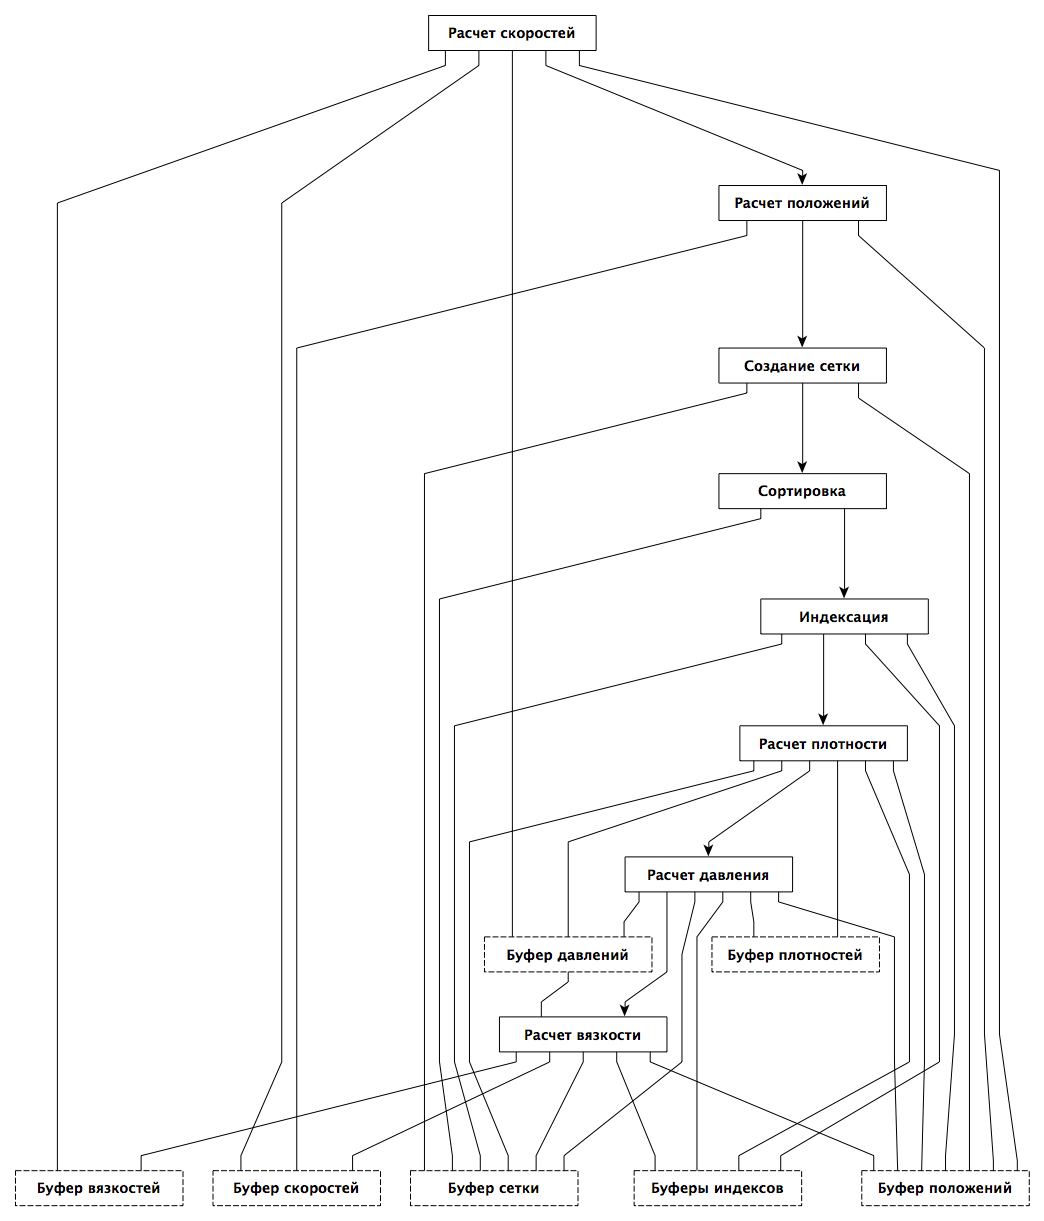
\includegraphics[scale=0.4]{Figures/buffers}
\end{center}
\caption{Зависимость между кадровыми буферами и программами}
\label{fig:buffers}
\end{figure}


\subsubsection{Поиск ближайших частиц}

В большинстве случаев частицы взаимодействуют друг с другом только если они находятся на 
заданном расстоянии. Т.е. определение соседних частиц ускоряет весь процесс симуляции.

Процесс определения соседних частиц занимает основное время всей симуляции. Существует
множество способов оптимизации. Ограничение объема, двоичное разбиение пространства, 
равномерная сетка, дискретизирующая пространство с целью улучшения производительности 
обнаружения соединений \cite{neisearch}.

В рамках данной работы реализован подход основанный на составлении сетки, модифицированный
под вычисления на графическом процессоре. Задача данного алгоритма поиск частиц входящих в 
радус $h$ текущей.

Разделение пространства -- один из подходов ускорения вычислений SPH величин.
Поиск потенциальных соединений осуществляется внутри ячеек сетки и между непосредственными 
соседями. Отсюда улучшение скорости всей симуляции. Алгоритм, используемый в данной работе
основан на данном принципе. 

Вычисление на GPU накладывает некоторые ограничения. Возникает это из-за того, что 
фрагментные шейдеры, которые используются как основной вычислительный блок не могут
писать в память по заданному адресу. Это ограничение усложняет многие основные
алгоритмические операции (подсчет, сортировка, поиск максимума, минимума).  

Один из подходов обойти данное ограничение -- разбить все пространство на ячейки, т.е.
хранить информацию о каждом участке в одной большой сетке.  \\

Детализация алгоритма:

\begin{enumerate}
  \item Вычисление одномерной координаты в сетке для каждой из частиц. Это достигается за счет
    дискретизации положения частицы до размеров сетки $h$ и получении целочисленных координат
    $(i_x, i_y, i_z)$. Полученные координаты конвертируются в одномерную с помощью следующего
    уравнения:

    \begin{equation}
    \label{eq:}
      i_x + i_y \times G_w + i_z \times G_w \times G_h,
    \end{equation}

    где $G_w$ -- ширина сетки, $G_h$ -- высота сетки.

  \item Одномерный индекс каждой координату записывается в буфер с указателями (uv-координатами)
    на каждую из частиц. Затем выполняется сортировка частиц по данным индексам.

  \item С помощью бинарного поиска для каждой частицы находится начальный индекс в сортированном
    буфере и записывается в другой буфер, который будет использоваться для доступа к ближайшим
    частицам.

  \item Поиск потенциальных соседей осуществляется следованием от первого индекса в сортированном
    буфере до следующего значения. По указателям, хранящимся рядом с индексом можно получить 
    информацию до любой величины (плотность, давление, скорость, положение и т.д.)

  \item Операция повторяется 27 раз (в трехмерном случае) проверяя соседние ячейки сетки.
    Благодаря тому что информация о начале каждого индекса хранится в специальном буфере,
    поиск выполняется один раз.

\end{enumerate}

Пример значений кадровых буфера при выполнении алгоритма изображен на рисунке \ref{fig:nei_search}.

\begin{figure}
\begin{center}
  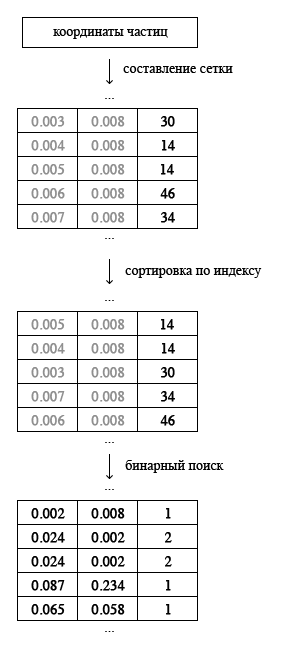
\includegraphics[scale=1]{Figures/nei_search}
\end{center}
\caption{Поиск ближайших частиц}
\label{fig:nei_search}
\end{figure}


\subsubsection{Сортировка}

Ввиду ограничений, накладываемых архитектурой графических процессоров, традиционные алгоритмы
сортировки (быстрая сортировка, сортировка вставками и т.п.) будут неэффективны. А передача
данных на ЦП крайне нежелательна.

Существенной особенностью алгоритмов для графических процессоров является их многопроходность
и параллельный характер. Задача увеличения эффективности сводится в уменьшению количества
проходов, необходимых для сортировки.

В данной работе используется алгоритм битонической сортировки. Он фокусируется на конвертации
последовательности случайных чисел в битоническую последовательность: которая сначала
монотонно увеличивается, а затем монотонно возрастает.

Битоническая сортировка может быть смоделирована как тип сортирующей сети. Начальная
не сортированная последовательность проходит через конвейер, где набор компараторов 
меняет местами значения в порядке возрастания или убывания.

Алгоритм сортировки состоит из двух операций: разделения и слияния.

Операция разделения -- процедура, которая разделяет одну битоническую последовательность на
две более мелкие. Причем элементы первой меньше или равны элементам второй.

Операция слияния -- вариация предыдущей: две смежных битонических последовательности
сливаются в одну и сортируются по возрастанию. Следующие две по убыванию и т.д. 
Две последовательности становятся одной битонической. Процедура повторяется до тех пор пока 
все входы сети полностью не покрыты. 

Пример сортирующей сети битонической сети для 16 входов изображена на рисунке \ref{fig:bitonic}.

\begin{figure}
\begin{center}
  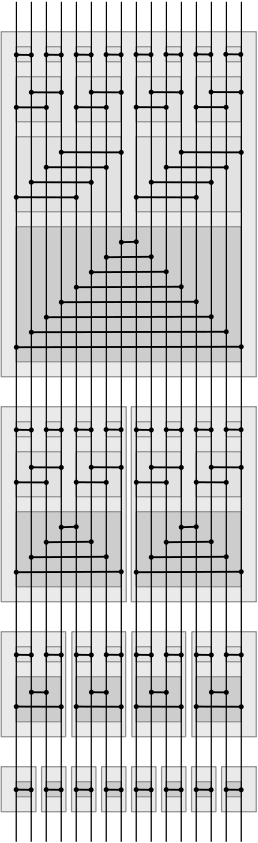
\includegraphics[scale=0.7]{Figures/bitonic}
\end{center}
\caption{Битоническая сортирующая сеть}
\label{fig:bitonic}
\end{figure}

